\documentclass{article}
\usepackage[utf8]{inputenc}
\usepackage[OT2]{fontenc}
\usepackage[serbianc, serbian]{babel}
\usepackage{hyperref}
\usepackage{graphicx}
\usepackage{minted}
\usepackage{xcolor} % to access the named colour LightGray
\definecolor{LightGray}{gray}{0.9}

\usepackage{float}

\title{Izveshtaj primene alata za verifikaciju nad bibliotekom za detekciju lica}
\author{Marija Eric1 \\ 
$marija.eric@matf.bg.ac.rs$}

\date{Januar 2023}


\begin{document}

\maketitle
\renewcommand{\abstractname}{Sazhetak}
\renewcommand*\contentsname{Sadrzhaj}



\begin{abstract}
Projekat na kome je izvrshena analiza je biblioteka za detekciju lica, napisana u $C++$. Biblioteka je otvorenog koda i mozhe se pronac1i na narednom \href{https://github.com/ShiqiYu/libfacedetection}{linku}. 
Primena alata je izvrshena na glavnoj grani, nad komitom chiji je hesh kod: $ec528ce43af9de94bf2fab308ce2d6270584881c$. U kodu nisu pronadjeni vec1i propusti, pored nekorish\-c1enih promenljivih i curenja memorije.
\end{abstract}
\tableofcontents
\newpage

\section{Verifikacija softvera}
\subsection{Dinamichka analiza}
\subsubsection{Izmena programa}
Da bismo mogli da repordukujemo rezultate dobijene prilikom izvrshavanja programa, neophodna je izmena u okviru $detect-camera$.
Na slici \ref{izmene} je prikazana izmena. Na levoj slici se nalazi originalan kod, a na desnoj izmenjeni kod.
\begin{figure}[H]
    \centering
    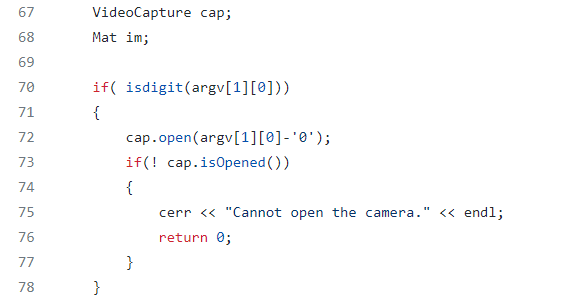
\includegraphics[width=6cm]{img/dc-original.png}
    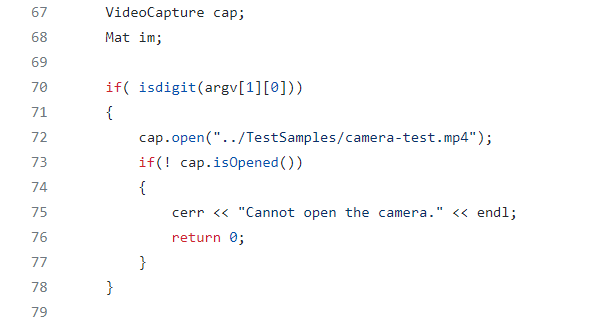
\includegraphics[width=6cm]{img/dc-izmena.png}
    
    \caption{Izmene u okviru $detect-camera$}
    \label{izmene}
\end{figure}

\subsubsection{$Gcov$}
$Gcov$ alat za odredivanje pokrivenosti koda prilikom
izvršavanja programa ($engl. code coverage$). Koristi se zajedno sa $gcc$ kompajlerom
da bi se analizirao program i utvrdilo kako se mozhe kreirati efikasniji, brzhi kod i da bi
se testovima pokrili delovi programa.
Zarad lepshe reprezentacije rezultata detekcije pokrivenosti koda izvrshavanjem test primera,
koristi se alat $lcov$ \cite{VSskripta}.

\paragraph{Nachin pokretanja alata:}
Prilikom kompilacije neophodno je koristiti dodatne opcije kompajlera koje
omoguc1avaju snimanje koliko je puta koja linija, grana i funkcija izvrshena. Detalji se nalaze na dnu teksta. U nastavku se nalazi pokretanje alata $lcov$ i generisanje $html$ izveshtaja.
\fontencoding{T1}\selectfont

\inputminted[firstline=5]{shell-session}{run_gcov.sh}

\fontencoding{OT2}\selectfont
Na slici \ref{covd:gcov} se nalazi izveshtaj za oba primera upotrebe biblioteke: $detect-image$ i $detect-camera.$ Analizirano je ispravno pokretanje programa. Kao shto vidimo pokrivenost koda je velika. Sve funkcije definisane u okviru biblioteke su iskorish\-c1ene. Pokrivenost grana je manja (oko 50\%). U okviru $detect-image$ i $detect-camera$ je velika pokrivenost naredbi. Jedine neizvrshene su naredbe obrade pogreshnog ulaza. Detaljan izveshtaj se mozhe videti na \ref{di:gcov} i \ref{dc:gcov}.
\begin{figure}[H]
    \centering
    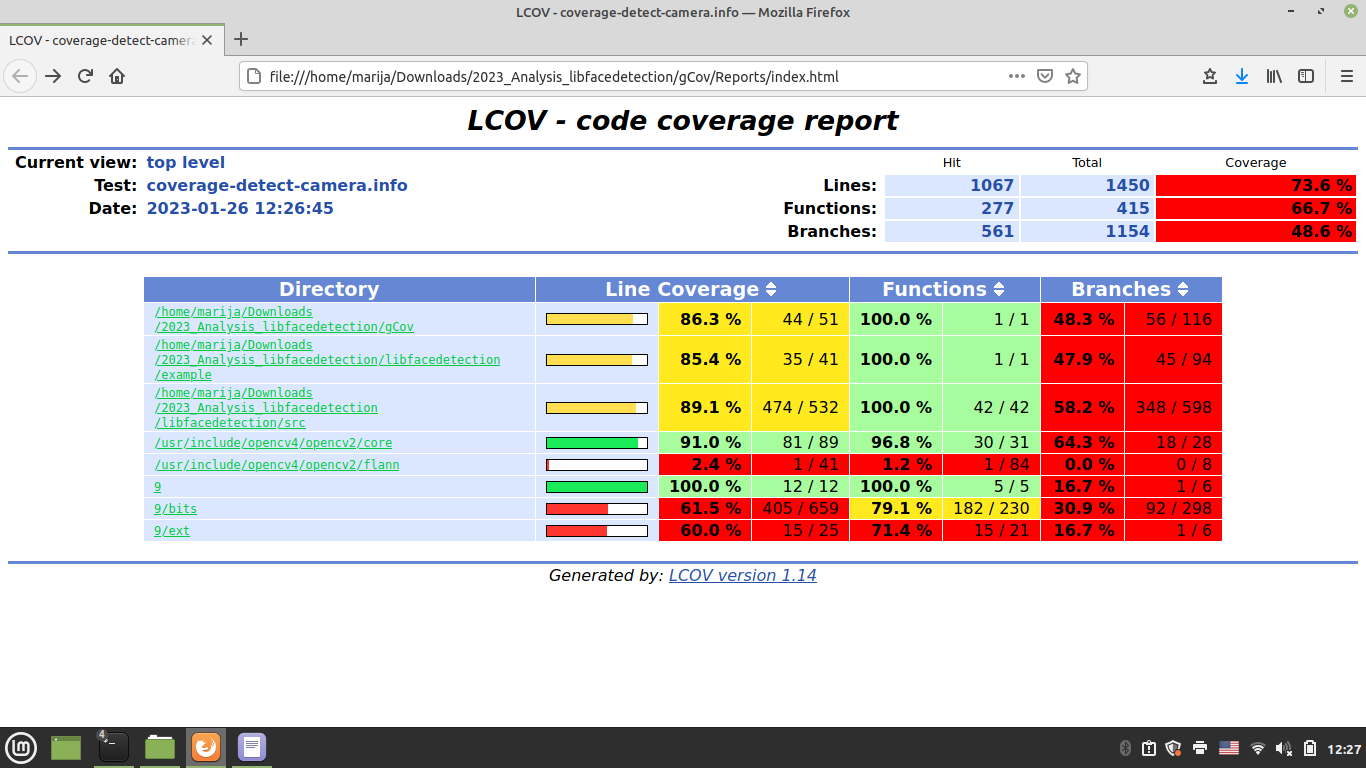
\includegraphics[width=12cm]{img/gcov/gcovCoverageDetect.png}
    \caption{Izveshtaj o pokrivenost koda}
    \label{covd:gcov}
\end{figure}

\paragraph{Rezultati:}

\begin{figure}[H]
    \centering
    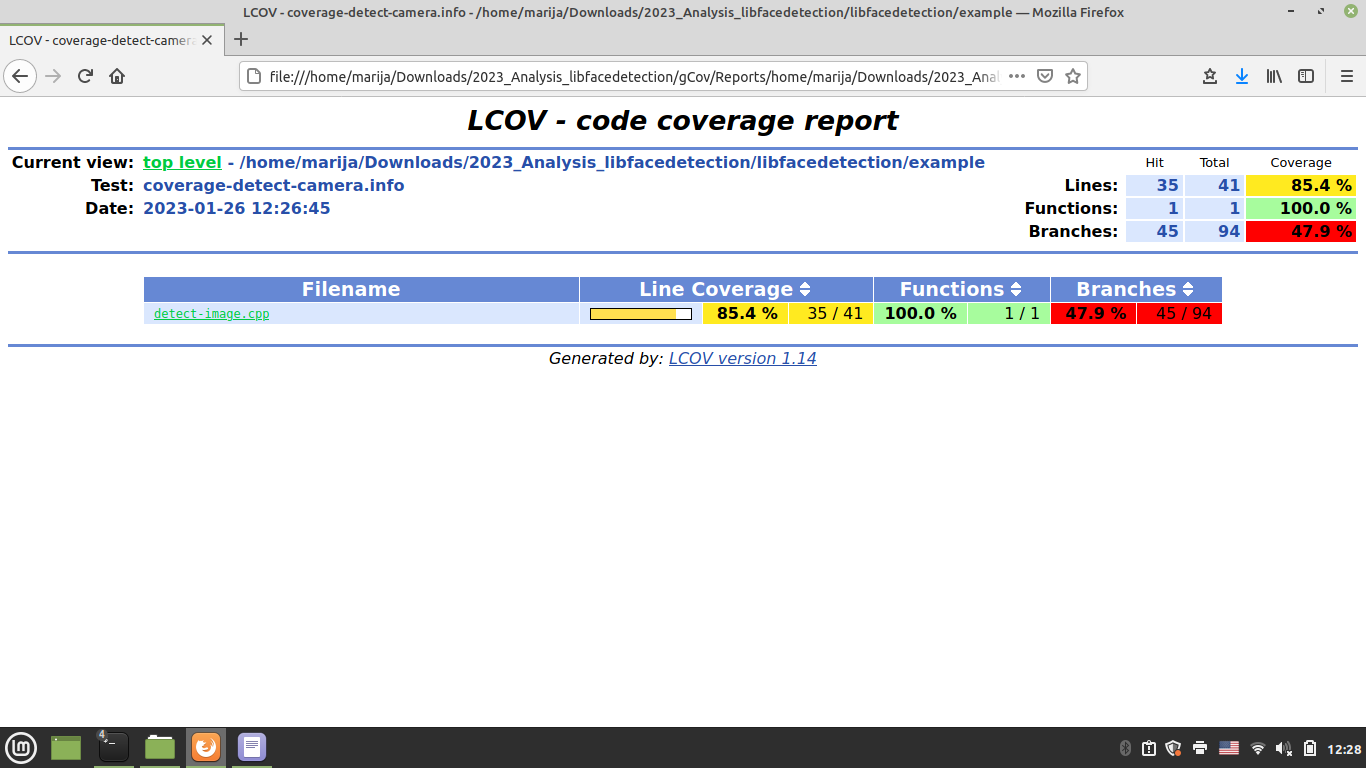
\includegraphics[width=12cm]{img/gcov/gcovDI.png}
    \caption{Pokrivenost koda $detect-image$}
    \label{di:gcov}
\end{figure}
\begin{figure}[H]
    \centering
    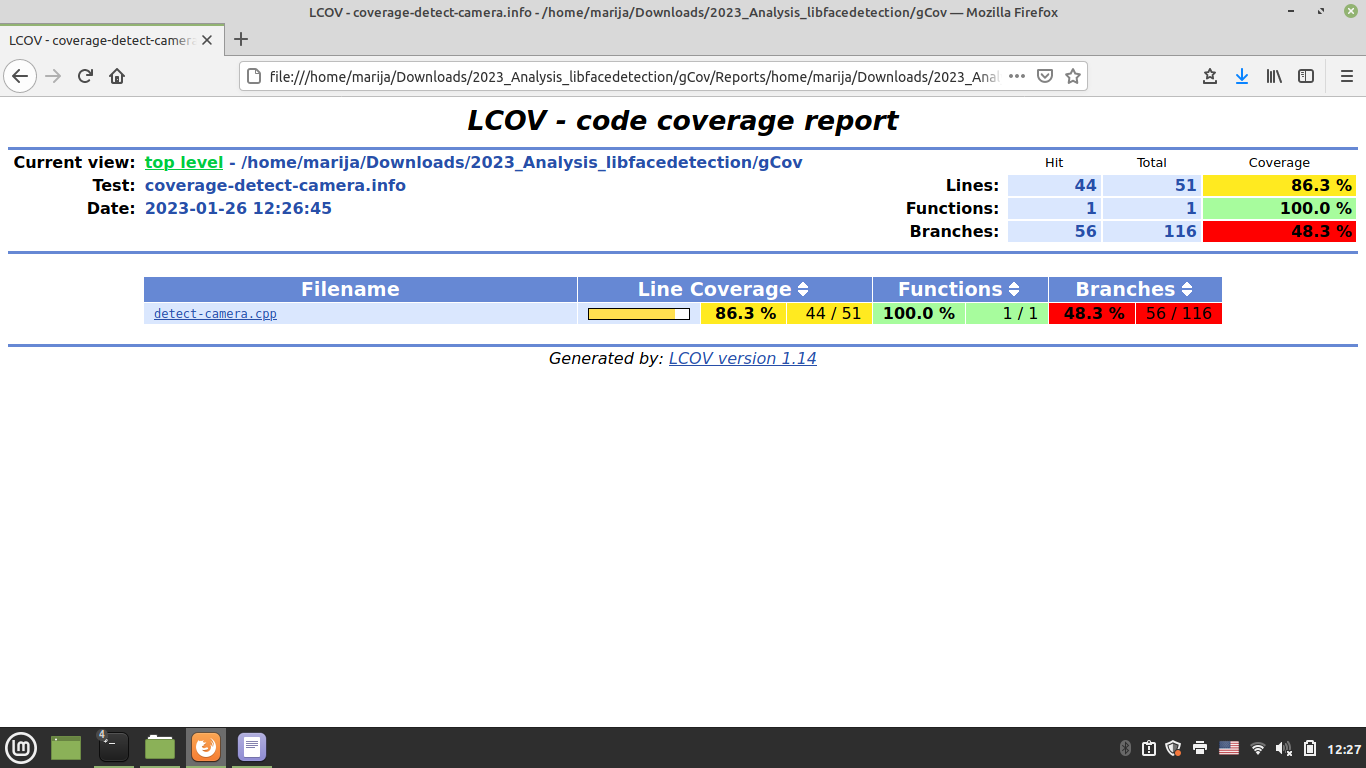
\includegraphics[width=12cm]{img/gcov/gcovDC.png}
    \caption{Pokrivenost koda $detect-camera$}
    \label{dc:gcov}
\end{figure}
\begin{figure}[H]
    \centering
    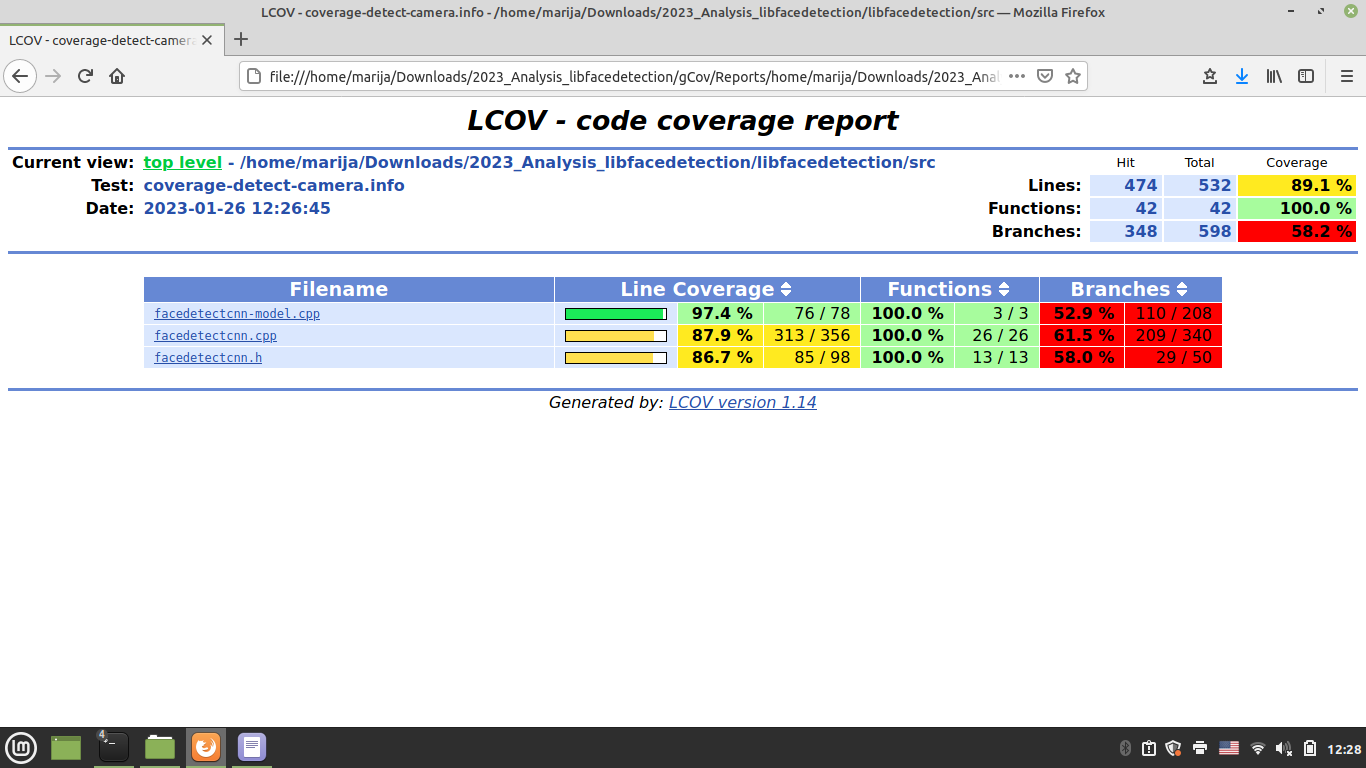
\includegraphics[width=12cm]{img/gcov/gcovSRC.png}
    \caption{Pokrivenost koda biblioteke }
    \label{src:gcov}
\end{figure}

Mala pokrivenost je u okviru $opencv$ biblioteke, jer se koristi samo jedna funkcija definisana u ovoj biblioteci, kao i funkcije iz $math$ biblioteke. 

Dakle, nakon pokretanja alata $gcov$ mozhemo da zakljuchimo da imamo veliku pokrivenost koda, kao i da nemamo nekorish\-c1ene funckije u okviru biblioteke za detekciju lica.

\subsection{Profajliranje}
Sa obzirom na to da se u okviru biblioteke koristi dinamichka alokacija memorije, bitno je da ispitamo da li je doshlo do curenja memorije. Iz tog razloga vrshimo profajliranje programa $detect-image$ i $detect-camera$. U okviru analize su korish\-c1eni alati $Memcheck$ i $Massif$.
\subsubsection{$Memcheck$}
%Uvod za memecheck%

\paragraph{Nachin pokretanja:} 
Bitno je da prevodjenje izvrshimo u $debug$ modu. Nakon toga, pokrec1eno $Memcheck$, deo izveshtaja je prikazan na slikama \ref{di:mcheck} i \ref{dc:mcheck}, dok se celokupan izlaz mozhe nac1i u okviru foldera $Memcheck$ na $github$ repozitorijumu. 
\fontencoding{T1}\selectfont
\inputminted[]{shell-session}{run_memcheck.sh}

\fontencoding{OT2}\selectfont
\begin{figure}[H]
    \centering
    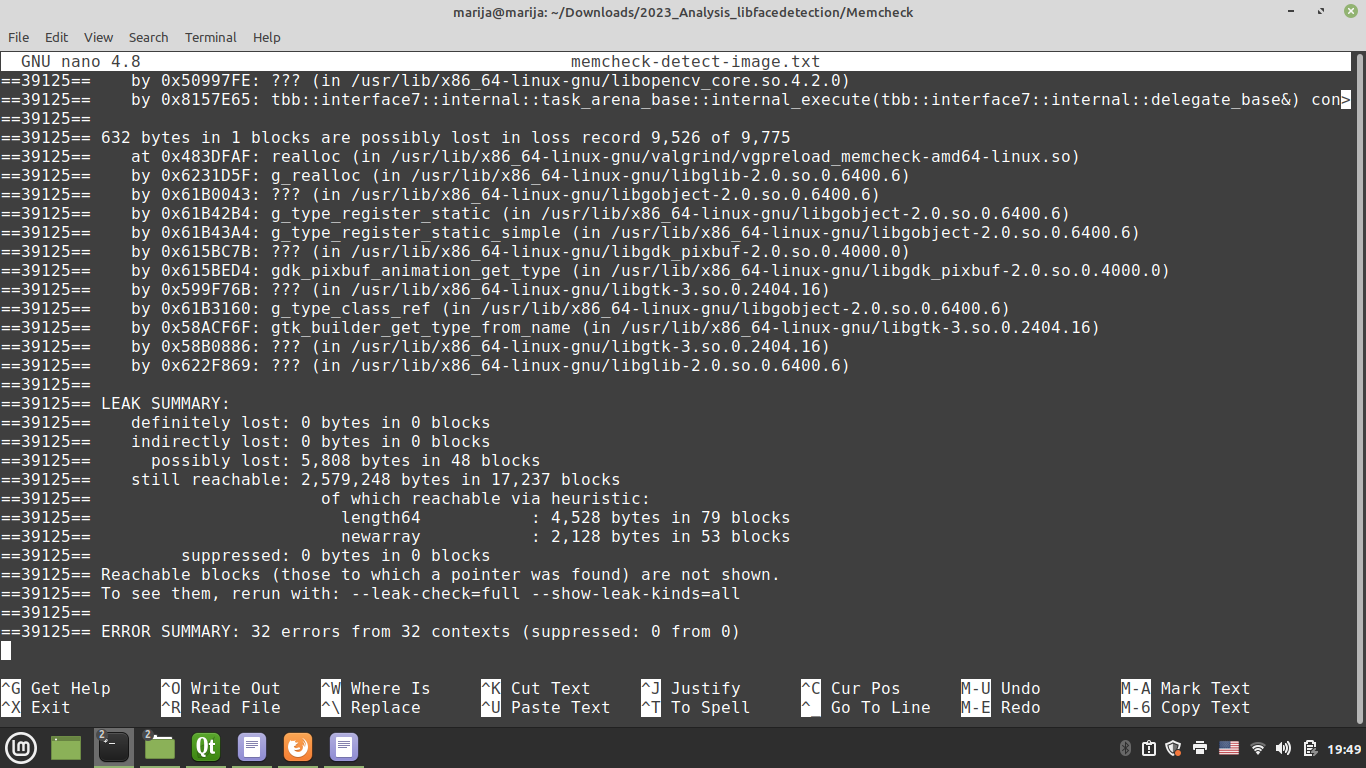
\includegraphics[width=12cm]{img/memcheck/memcheck-detect-image.png}
    \caption{Deo izlaza alata $Memcheck$ nad $detect-image.$}
    \label{di:mcheck}
\end{figure}

\begin{figure}[H]
    \centering
    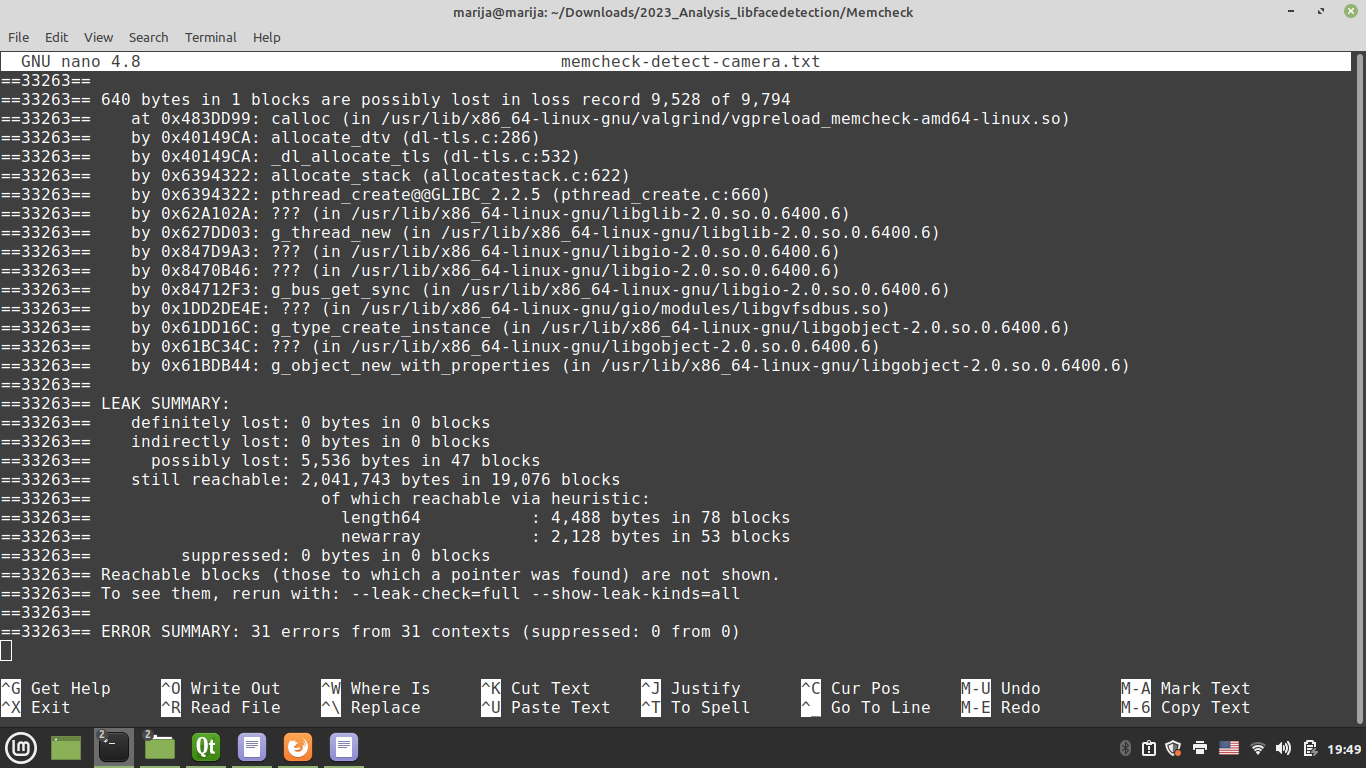
\includegraphics[width=12cm]{img/memcheck/memcheck_detect_camera.png}
    \caption{Deo izlaza alata $Memcheck$ nad $detect-camera.$}
    \label{dc:mcheck}
\end{figure}
Dobijamo jako slichne izlaze za oba programa. Na osnovu sazhetka alata vidimo da nema curenja memorije. 
Takođe vidimo da imamo moguc1i gubitak (oko 5000 bajtova u oba programa). Kada ispitamo stek poziva vidimo da je moguc1i gubitak izazvao poziv funkcije $calloc$, ali zakljuchujemo da ne postoji gubitak memorije koji je izazvan od strane programera.
\subsubsection{$Massif$}
\fontencoding{OT2}\selectfont
$Massif$ predstavlja profajler $heap$ memorije. Ovaj alat meri koliko $heap$ memorije program koristi (korisna memorije + dodatna memorija za administraciju). U okviru ove analize je merena i velichina steka korish\-c1ena u okviru programa.

Motivacija iza korishc1enja i ovog alata lezhi u tome da Memcheck ne mozhe da detektuje sva potencijalna curenja memorije.

\fontencoding{T1}\selectfont
\inputminted[fistline=3, lastline=6]{shell-session}{run_massif.sh}
\fontencoding{OT2}\selectfont
Za vizuelizaciju rezultata korish\-c1en $massif-visualizer$, koji je preuzet sa \href{https://github.com/KDE/massif-visualizer}{$https://github.com/KDE/massif-visualizer$}, gde se mozhe pronac1i detaljno uput\-stvo za instaliranje i pokretanje.

Na slikama \ref{dim:massif} i \ref{dima:massif} se nalaze izveshtaji vezani za program $detect-image$, dok se na slikama \ref{dcm:massif} i \ref{dcma:massif} nalaze izveshtaji vezani za program $detect-camera$. 

\begin{figure}[H]
    \centering
    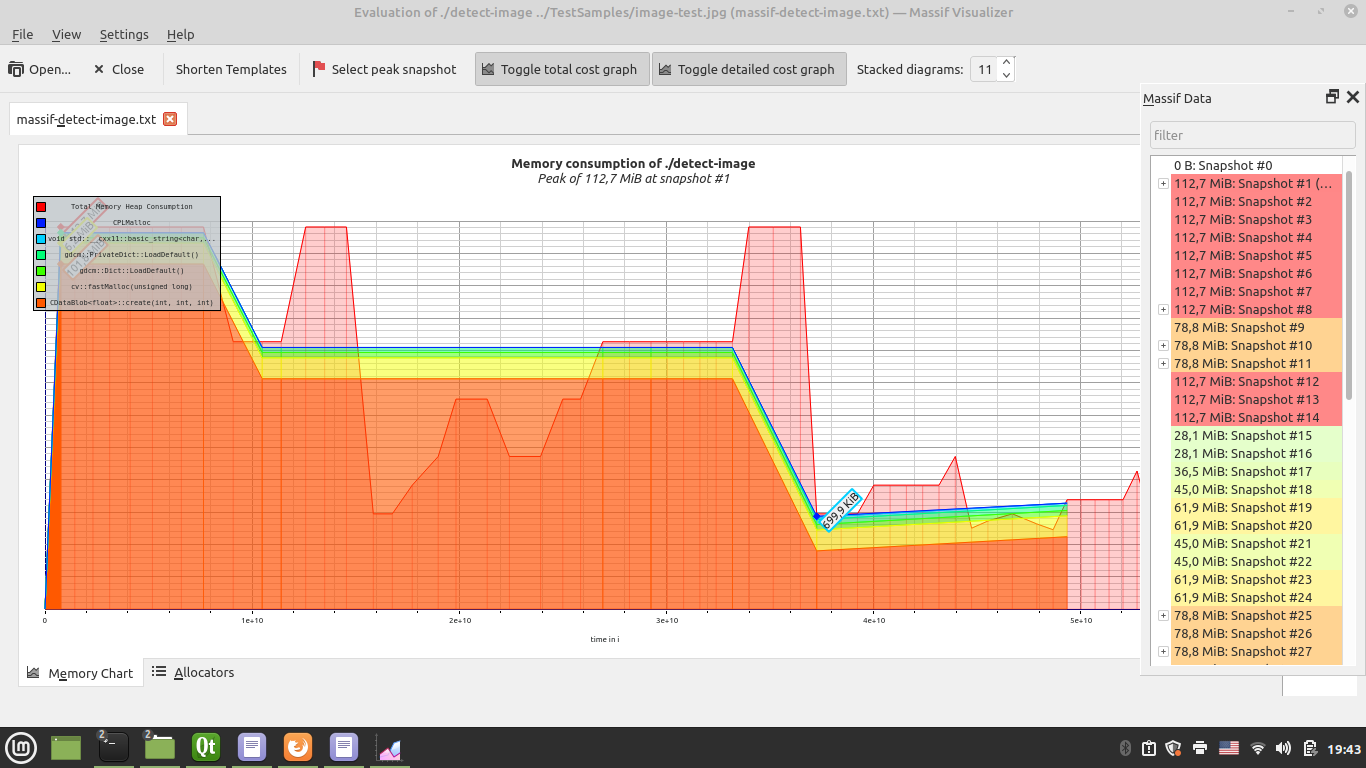
\includegraphics[width=12cm]{img/massif/massif_detect_image_memory.png}
    \caption{Korish\-c1enje memorije u programu $detect-image$}
    \label{dim:massif}
\end{figure}
\begin{figure}[H]
    \centering
    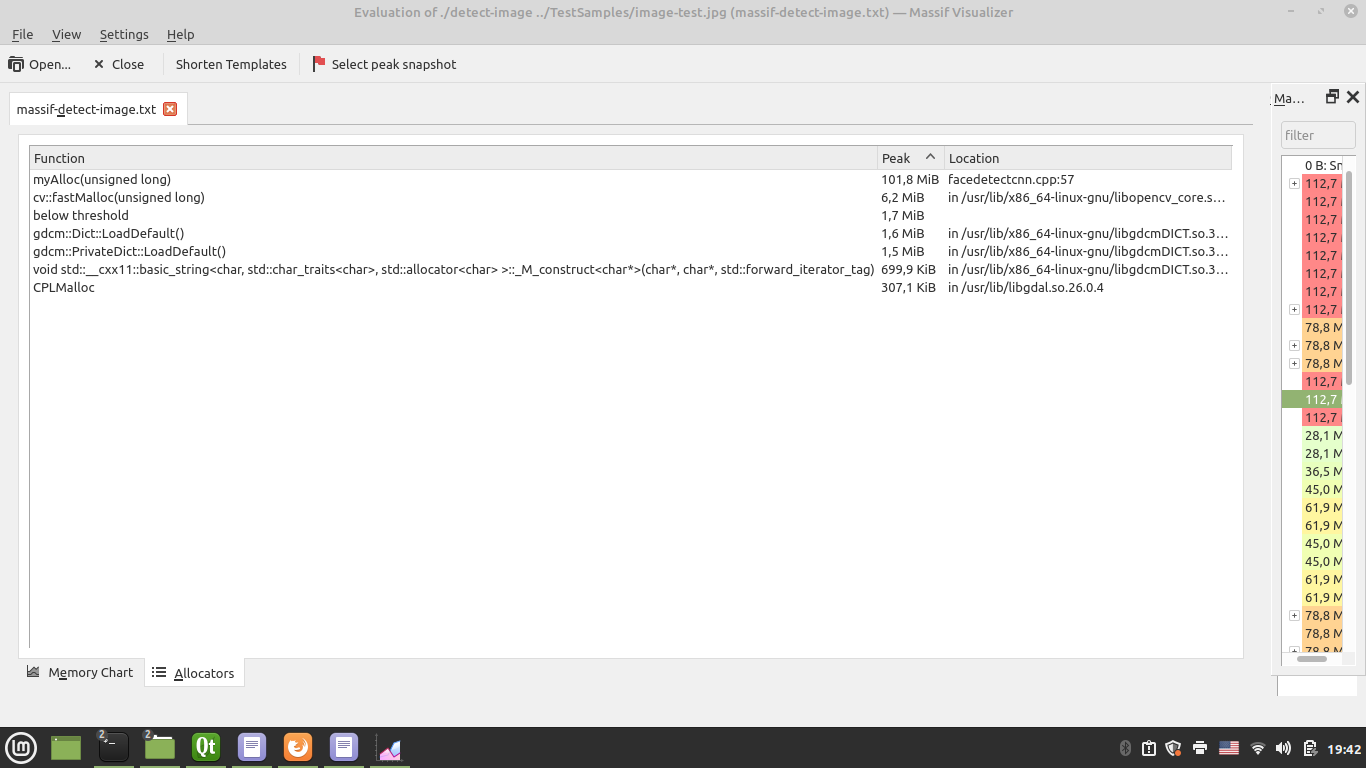
\includegraphics[width=12cm]{img/massif/massif_detect_image_allocators.png}
    \caption{Alokatori u programu $detect-image$}
    \label{dima:massif}
\end{figure}

Na slici \ref{dim:massif} mozhemo videti stanje $heap-a$ tokom izvrshavanja programa $detect-image$.  Vidimo da se na pochetku izvrshavanja vrshi alociranje memorije koja c1e se koristiti u nastavku, i $peak$ se deshava u nekoliko prvih $snapshotova.$ Nakon toga se samo vrshu dealokacija memorije. Jedan od grafika sa slike koji ima velike skokove predstavlja ukupnu korish\-c1enu memoriju (zajedno sa stekom), pa ima dosta promena.


\begin{figure}[H]
    \centering
    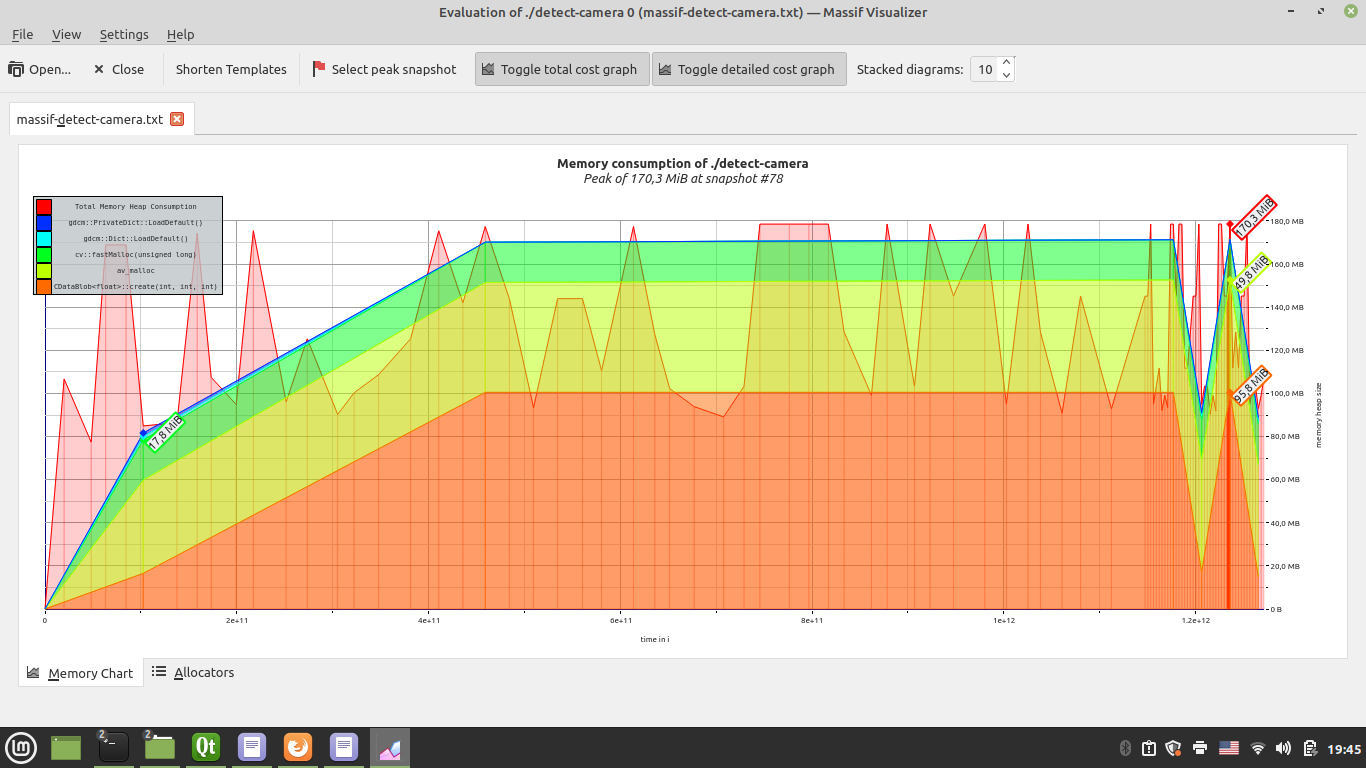
\includegraphics[width=12cm]{img/massif/massif_detect_camera_memory1.png}
    \caption{Korish\-c1enje memorije u programu $detect-camera$}
    \label{dcm:massif}
\end{figure}

\begin{figure}[H]
    \centering
    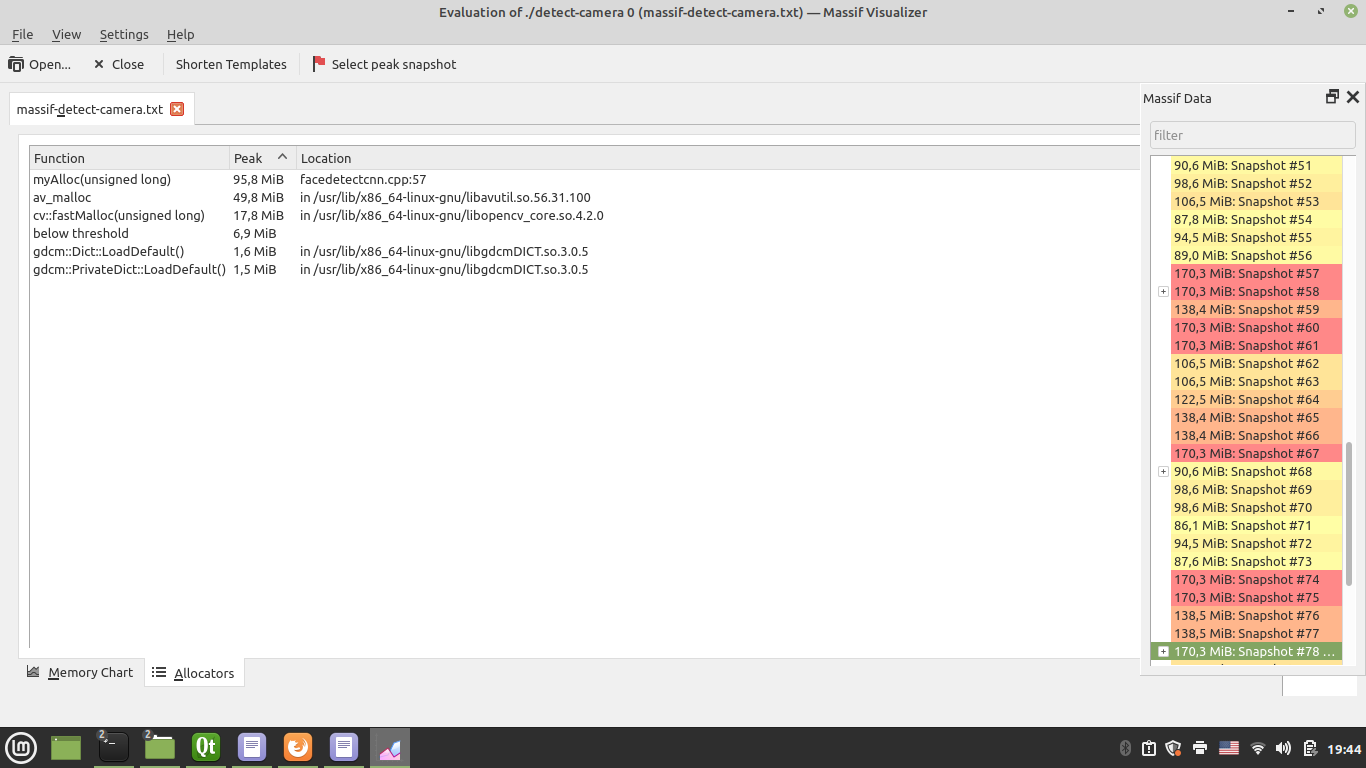
\includegraphics[width=12cm]{img/massif/massif_detect_camera_allocators.png}
    \caption{Alokatori u programu $detect-camera$}
    \label{dcma:massif}
\end{figure}


Na slici \ref{dcm:massif} je prikazao stanje $heapa$ tokom izvrshavanja programa $detect-camera.$
Situacija je slichna kao kod programa $detect-image.$ Nakon detekcije lica na jednoj slici, vrshi se dealokacije. Taj sluchaj je uhvac1en u okviru $snapshota 68.$

Na osnovu gorenavedenih komentara mozhemo zakljuchiti da je odgovrno korishc1en $heap$.
\subsection{Statichka analiza}
\subsubsection{$CppCheck$}
$CppCheck$ je alat za statichku analizu $C/C++$ koda, koji pruzha jedinstvenu analizu za detekciju greshaka, sa fokusom na nedefinisano ponashanje i sa opasnim konstruktima koda. Analiza dobijena $CppCheck$ nije ni saglasna, niti je potpuna. Dakle, mozhe imati i lazhno pozitivne rezultate, kao i lazhno negativne.
Moguc1e poruke:
\begin{itemize}
    \item Greshka - nedefinisano ponashanje (curenje memorije ili curenje resursa)
    \item Stil - redundantnost, nekorish\-c1ene funkcije/promenljive, potencijalne greshke
    \item Performanse - popravka ovih poruka ne garantuje ubrzanje (jer je statichka analiza u pitanju)
    \item Prenosivost
    \item Konfiguracione informacije
\end{itemize}
\paragraph*{Instaliranje i pokretanje alata:}
Detaljna instalacija 
\href{https://cppcheck.sourceforge.io/}{zvanichnoj stranici.} 
Detaljan opis nachina korish\-c1enja alata se mozhe nac1i u \cite{cppCheckMan}.

Prilikom instalacije na Debian distribuciji:
\fontencoding{T1}\selectfont
\begin{minted}{shell-session}
sudo apt-get install cppcheck
\end{minted}

\fontencoding{OT2}\selectfont
Pokretanje alata $cppcheck$ nad projektom $libfacedetection$: 

\fontencoding{T1}\selectfont
\begin{minted}{shell-session}
cppcheck --enable=all --output-file="cppCheckOut.xml" --xml
--inconclusive libfacedetection/
\end{minted}

\fontencoding{OT2}\selectfont
Dodatni flagovi:\\
$--enable = all$ - pronalazak svi greshaka \\
$--output-file$ - definisanje fajla u koji se upisuje \\
$--xml$ - poruke u $xml$ formatu \\
$--inconclusive$ - neuverljive greshke (potencijalni $false$ $positive$)
\\
U okviru alata je moguc1e napraviti $HTML report$ od izlazne poruke sachuvane u $xml$ formatu. 

\fontencoding{T1}\selectfont
\begin{minted}{shell-session}
cppcheck-htmlreport --report-dir=CppCheckReport --output-file="cppCheckOut.xml" 
\end{minted}

\fontencoding{OT2}\selectfont

Skripta za pokretanje alata se nalazi na $github$; u okviru $README$.

Prikaz pokretanja u alata: \ref{msg:cppcheck}

\begin{figure}[H]
    \centering
    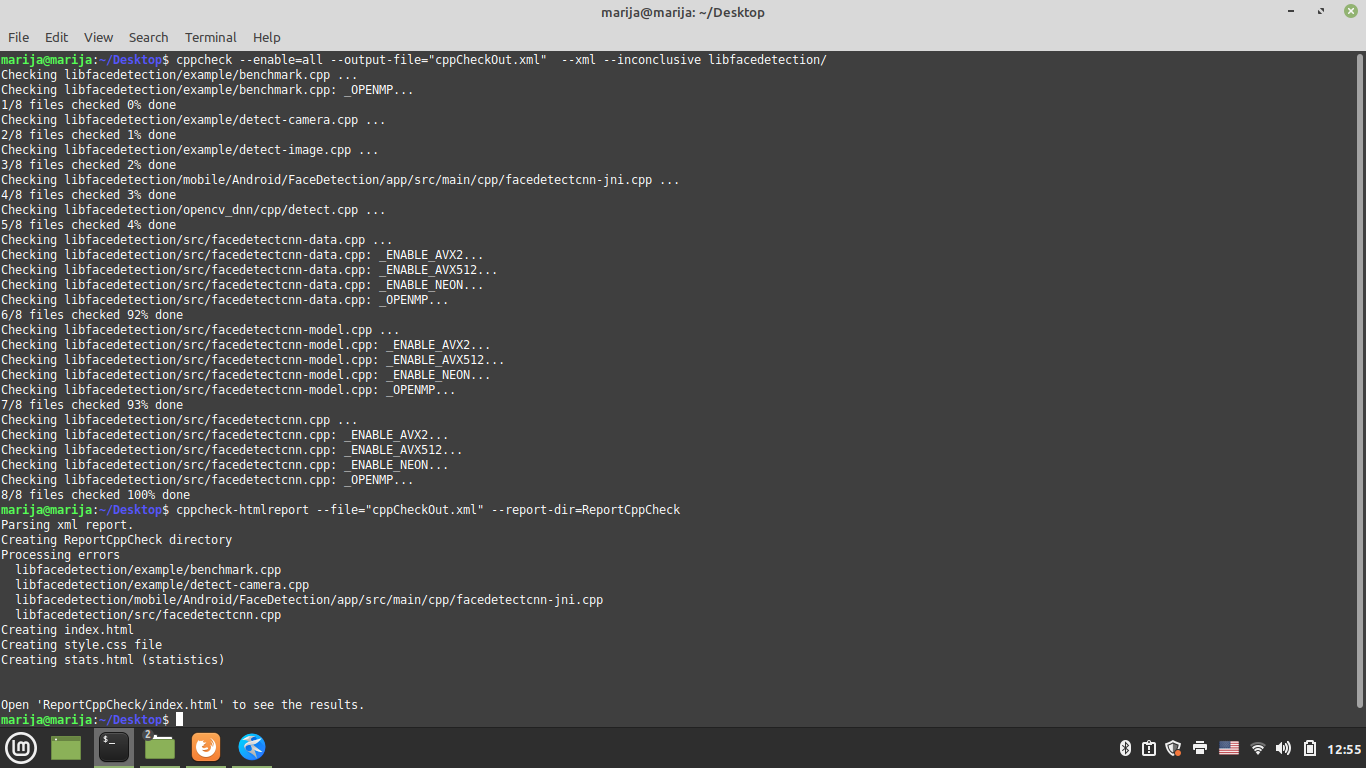
\includegraphics[width=12cm]{img/cppCheck/cppCheckTerminal.png}
    \caption{Poruka o gresh\-ci u $cppCheck$}
    \label{msg:cppcheck}
\end{figure}
%----------------------------------------------------------------%
\paragraph{Rezultati analize:}
Na slici \ref{stats:cppcheck} se nalazi statistika analize.

\begin{figure}[H]
    \centering
    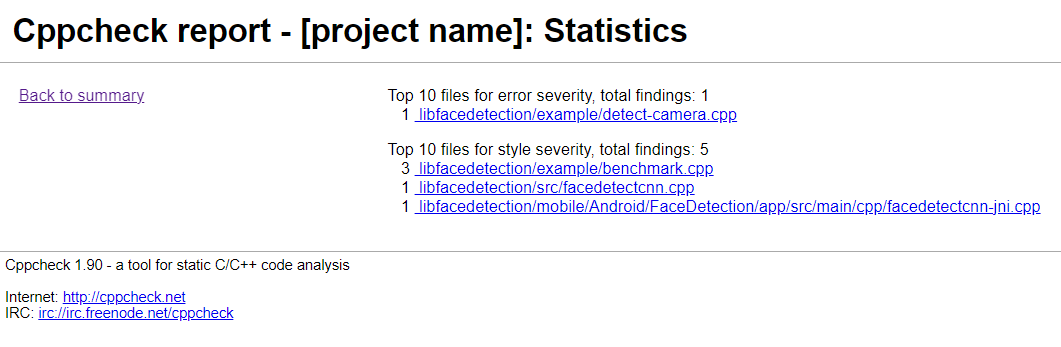
\includegraphics[width=12cm]{img/cppCheck/cppCheckStats.png}
    \caption{Statistika analize alata $cppcheck$}
    \label{stats:cppcheck}
\end{figure}
Na osnovu statistike vidimo da je pronadjena jedna poruka tipa \textit{greshka}, i 5 poruka tipa \textit{stil}.

Detaljnije o porukama se mozhe videti na slici \ref{html:cppcheck}.
\begin{figure}[H]
    \centering
    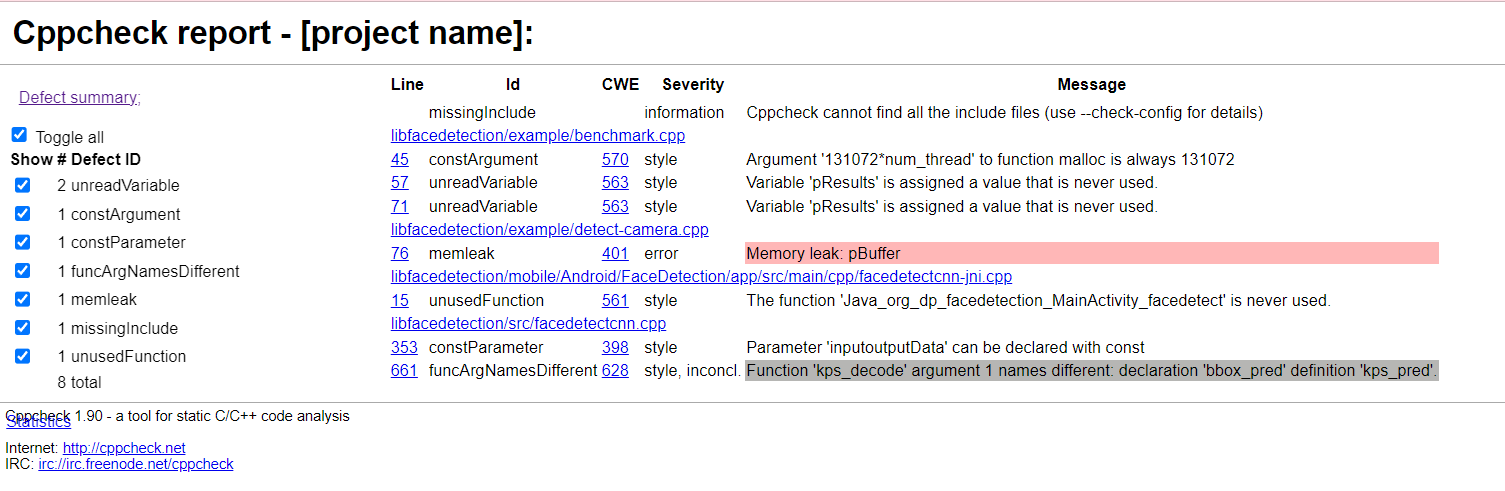
\includegraphics[width=12cm]{img/cppCheck/cppChechHtmlReport.png}
    \caption{Izveshtaj alata $cppcheck$}
    \label{html:cppcheck}
\end{figure}

Greshka se nalazi u 76 liniji u fajlu $detect-camera.cpp$. Deo koda koji izaziva greshku je dat u nastavku:
\fontencoding{T1}\selectfont

\inputminted[frame=lines,
framesep=2mm,
baselinestretch=1.2,
bgcolor=LightGray,
fontsize=\footnotesize,
firstline=55,
lastline=77,
linenos
]{cpp}{detect-camera.cpp}

\fontencoding{OT2}\selectfont
Dakle, memorija koje je alocirana u liniji 59 se ne oslobadja pre prekida izvrshavanja programa, ukoliko je $VideoCapture$ neuspeshno otvoren.

Pored toga su prijavljena upozrorenja za nekorish\-c1ene promenljive i funkcije. Detaljan izveshtaj se mozhe pronac1i u okviru repozitorijuma za analizu projekta, u okviru foldera $CppCheckReport.$ U navedenom repozitorijumu je za svaki fajl u kome je alat pronashao neki problem napravljen $html$ izveshtaj sa obelezhenim mestima sa pronadjenim problemima.


\fontencoding{OT2}\selectfont
Takodje, moguc1e je pokretanje alata u okviru razvojnog okrizhenja $QtCreator.$ Poshto nije 
\fontencoding{T1}\selectfont
\textbf{Help->About Plugins -> Code Analyzer}.
\fontencoding{OT2}\selectfont
Izabrati $Cppcheck$. Nakon toga 
je neophodno restartovanje okruzhenje.

Nakon toga: 
\fontencoding{T1}\selectfont
\textbf{Analyze -> Cppcheck}
\fontencoding{OT2}\selectfont
nakon chega se otvara prozor prikazan na slici \ref{qt:cppcheck}.

\begin{figure}[H]
    \centering
    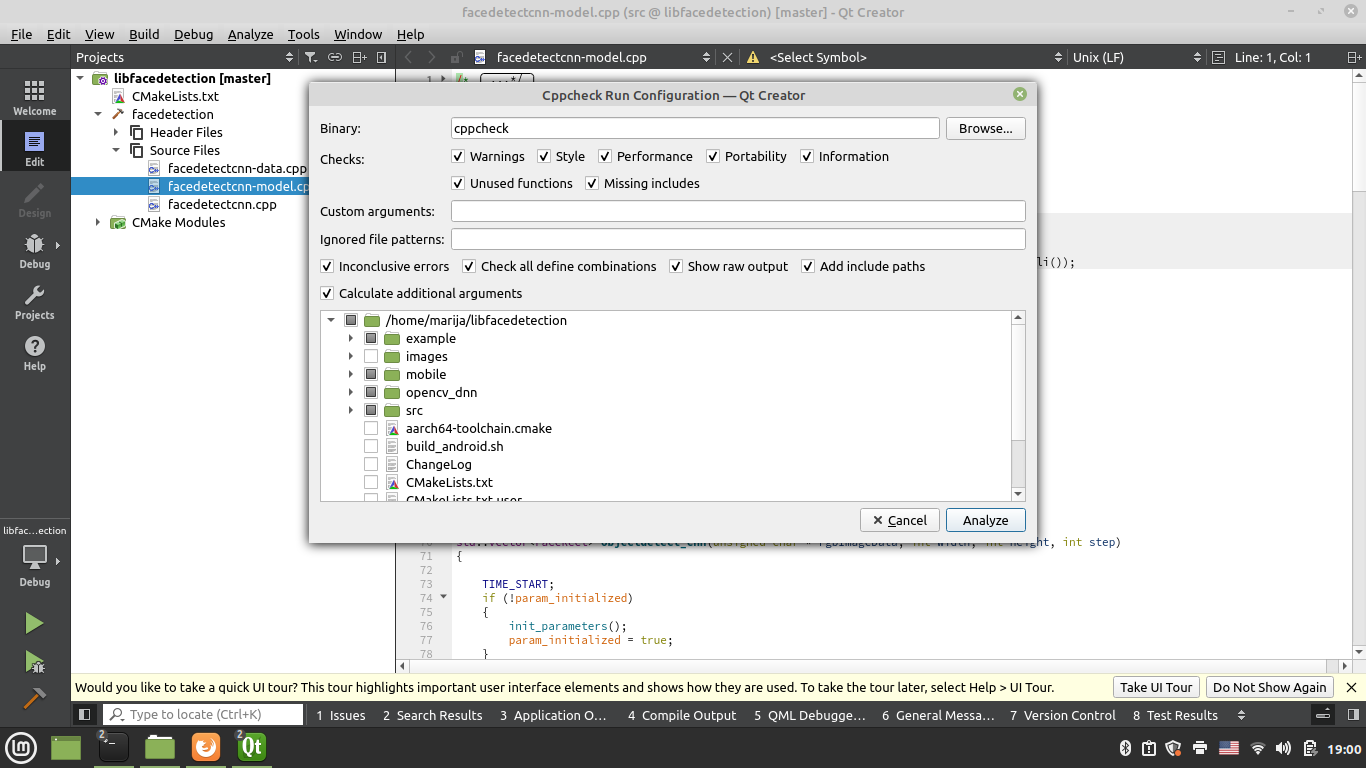
\includegraphics[width=10cm]{img/cppCheck/cppCheckQt.png}
    \caption{Pokretanje alata u okviru $QtCreatora$}
    \label{qt:cppcheck}
\end{figure}

Selektovanjem polja $inconclusive$ $errors$ se prijavljuju i lazhna upozorenja ($false$ $positive$). 

\section{Zakljuchak}
U okviru projekta je analizirana biblioteka za detekciju lica i dva njena primera upotrebe - detekcija lica na prosled1enoj slici i detekcija lica sa kamere uredjaja. Korish\-c1ena su chetiri alata za analizu. Na osnovu njih mozhemo zakljuchiti da biblioteka nema vec1ih propusta. Dinamichkom analizom nisu pronadjeni propusti, dok je statichka analiza pronashla curenje memorije i nekoliko nekorish\-c1enih promenljivih.

\section{Pokretanje skripti za reprodukovanje rezultata}
\fontencoding{T1}\selectfont


\begin{minted}{shell-session}
git clone https://github.com/MATF-Software-Verification/2023_Analysis_libfacedetection
cd 2023_Analysis_libfacedetection/libfacedetection
git submodule init
git submodule update
\end{minted}

\subsection*{Prevodjenje biblioteke}

\begin{minted}{shell-session}
cd libfacedetection
mkdir build
cd build
cmake .. -DCMAKE_INSTALL_PREFIX=install 
-DBUILD_SHARED_LIBS=ON -DCMAKE_BUILD_TYPE=Debug -DDEMO=OFF
cmake --build . --config Debug
cmake --build . --config Debug --target install
\end{minted}

\subsection{Pokretanje alata}
\fontencoding{OT2}\selectfont
Pre pokretanja alata potrebno je preuzimanje projekta i prevodjenje biblioteke. \\
Nakon toga je potrebno prevesti programe $detect-image$ i $detect-camera$:
\fontencoding{T1}\selectfont
\begin{minted}{shell-session}
cd ../TestSamples
bash build.sh
\end{minted}

\subsection*{$CppCheck$}
\begin{minted}{shell-session}
cd ../CppCheckReport
bash run_cppcheck.sh
\end{minted}

\subsection*{$Gcov$}
\begin{minted}{shell-session}
cd ../CppCheckReport
bash run_gcov.sh
\end{minted}

\subsection*{$Memcheck$}
\begin{minted}{shell-session}
cd ../Memcheck
bash run_memcheck.sh
\end{minted}
\subsection*{$Massif$}
\begin{minted}{shell-session}
cd ../Massif
bash run_massif.sh
\end{minted}
\newpage
\fontencoding{OT2}\selectfont

\bibliographystyle{plain}
\fontencoding{T1}\selectfont
\bibliography{literatura}

\end{document}
